\documentclass[aspectratio=169, 10pt]{beamer}

% Paquetes esenciales
\usepackage[utf8]{inputenc}
\usepackage[spanish, es-tabla]{babel}
\usepackage{graphicx}
\graphicspath{{img/}{./}}
\usepackage{booktabs}
\usepackage{tabularx}
\usepackage{tikz}
\usepackage{hyperref}

% Estilo visual limpio y moderno
\usetheme{default}
\usefonttheme{structurebold}

% Colores basados en la identidad institucional UCN
\definecolor{ucnblue}{RGB}{11, 44, 76}      % Azul marino institucional
\definecolor{ucnaccent}{RGB}{0, 119, 182}   % Azul acento
\definecolor{ucngray}{RGB}{242, 246, 250}   % Fondo de tarjetas
\definecolor{darktext}{RGB}{30, 41, 59}     % Texto principal oscuro

\setbeamercolor{normal text}{fg=darktext}
\setbeamercolor{structure}{fg=ucnblue}
\setbeamercolor{title}{fg=ucnblue}
\setbeamercolor{block title}{fg=white, bg=ucnblue}
\setbeamercolor{block body}{fg=darktext, bg=ucngray}
\setbeamercolor{block title example}{fg=white, bg=ucnaccent}
\setbeamercolor{block body example}{fg=darktext, bg=ucngray}

% Quitar iconos de navegacion de Beamer
\setbeamertemplate{navigation symbols}{}

% Encabezado limpio de diapositiva
\setbeamertemplate{frametitle}{
    \vspace{0.25cm}
    {\Large \textbf{\insertframetitle}}
    \par\vspace{0.1cm}
    \textcolor{ucnaccent}{\rule{\textwidth}{0.8pt}}
    \vspace{-0.1cm}
}

% Pie de pagina sencillo con numeracion
\setbeamertemplate{footline}{%
    \leavevmode%
    \begin{beamercolorbox}[wd=\paperwidth,ht=2.5ex,dp=1ex]{footline}%
        \hspace*{0.5cm}\scriptsize \textcolor{gray}{Ingeniería de Datos y Big Data · Entrega 2: ETL y Data Warehouse}%
        \hfill%
        \scriptsize \textcolor{gray}{\insertframenumber{} / \inserttotalframenumber}%
        \hspace*{0.6cm}%
    \end{beamercolorbox}%
    \vskip3pt%
}

% Informacion de la presentacion
\title{Proyecto de Reportabilidad (ETL)}
\subtitle{Entregable 2: Proceso ETL, Data Warehouse y Diseño Final de Reportes}
\author{Martín Castillo Torrejón · Daniel Durán García}
\institute{
    Escuela de Ingeniería · Sede Coquimbo\\
    Ingeniería en Tecnologías de Información\\
    Universidad Católica del Norte
}
\date{Lunes 28 de Septiembre de 2026}

\begin{document}

% -----------------------------------------------------------------------
% SLIDE 1: PORTADA
% -----------------------------------------------------------------------
\begin{frame}[plain]
    \vspace{0.2cm}
    \noindent
    
\includegraphics[height=1.3cm]{UCN.png} \hfill 
\includegraphics[height=1.3cm]{EIC.png}
    
    \vspace{0.6cm}
    \centering
    {\LARGE \textbf{\textcolor{ucnblue}{Proyecto de Reportabilidad (ETL)}}}\\[0.25cm]
    {\large \textbf{Entregable 2: Base de Datos OLAP, Tareas de ETL y Diseño de Reportes}}\\[0.6cm]
    
    \textbf{Martín Castillo Torrejón · Daniel Durán García}\\[0.15cm]
    \footnotesize Escuela de Ingeniería · Sede Coquimbo · Universidad Católica del Norte\\[0.4cm]
    
    \scriptsize \textcolor{gray}{Repositorio del Proyecto: \url{https://github.com/Charmandiox9/Ing.-Datos-y-Big-Data}}
\end{frame}

% -----------------------------------------------------------------------
% SLIDE 2: OBJETIVOS DEL ENTREGABLE 2
% -----------------------------------------------------------------------
\begin{frame}{Objetivos del Entregable 2}
    En esta segunda etapa del proyecto se cumplen los tres requerimientos centrales solicitados:
    
    \vspace{0.3cm}
    \begin{columns}[t]
        \begin{column}{0.31\textwidth}
            \begin{block}{1. Base de Datos OLAP}
                \small
                \begin{itemize}
                    \item Almacén analítico implementado en SQL Server.
                    \item Base de datos independiente: \texttt{AdventureWorksDW}.
                    \item Modelo dimensional en estrella operativo.
                \end{itemize}
            \end{block}
        \end{column}
        
        \begin{column}{0.31\textwidth}
            \begin{block}{2. Tareas de ETL}
                \small
                \begin{itemize}
                    \item Proceso de extracción, transformación y carga.
                    \item Automatizado mediante scripts SQL y PowerShell.
                    \item Limpieza y tolerancia ante datos erróneos.
                \end{itemize}
            \end{block}
        \end{column}
        
        \begin{column}{0.31\textwidth}
            \begin{block}{3. Diseño de Reportes}
                \small
                \begin{itemize}
                    \item Catálogo final de 15 reportes en tres áreas clave.
                    \item 15 vistas SQL (\texttt{rpt}) listas para conectar.
                    \item Preparado para la Entrega 3 en Power BI.
                \end{itemize}
            \end{block}
        \end{column}
    \end{columns}
\end{frame}

% -----------------------------------------------------------------------
% SLIDE 3: FUENTE TRANSACCIONAL (OLTP)
% -----------------------------------------------------------------------
\begin{frame}{Base de Datos de Origen (OLTP)}
    \begin{columns}[c]
        \begin{column}{0.52\textwidth}
            \begin{block}{Situación de la Fuente}
                \small
                \begin{itemize}
                    \item \textbf{Origen:} \texttt{AdventureWorks2022} restaurada en SQL Server sobre contenedor Docker.
                    \item \textbf{Estructura:} Base transaccional normalizada con esquemas \texttt{Sales}, \texttt{Production}, \texttt{Purchasing} y \texttt{Person}.
                    \item \textbf{Problema:} Más de 68 tablas con relaciones complejas. Consultar directo sobre ella ralentiza el sistema y dificulta armar gráficos.
                    \item \textbf{Solución:} Separar los datos operacionales de los datos analíticos en una base propia.
                \end{itemize}
            \end{block}
        \end{column}
        
        \begin{column}{0.45\textwidth}
            \centering
            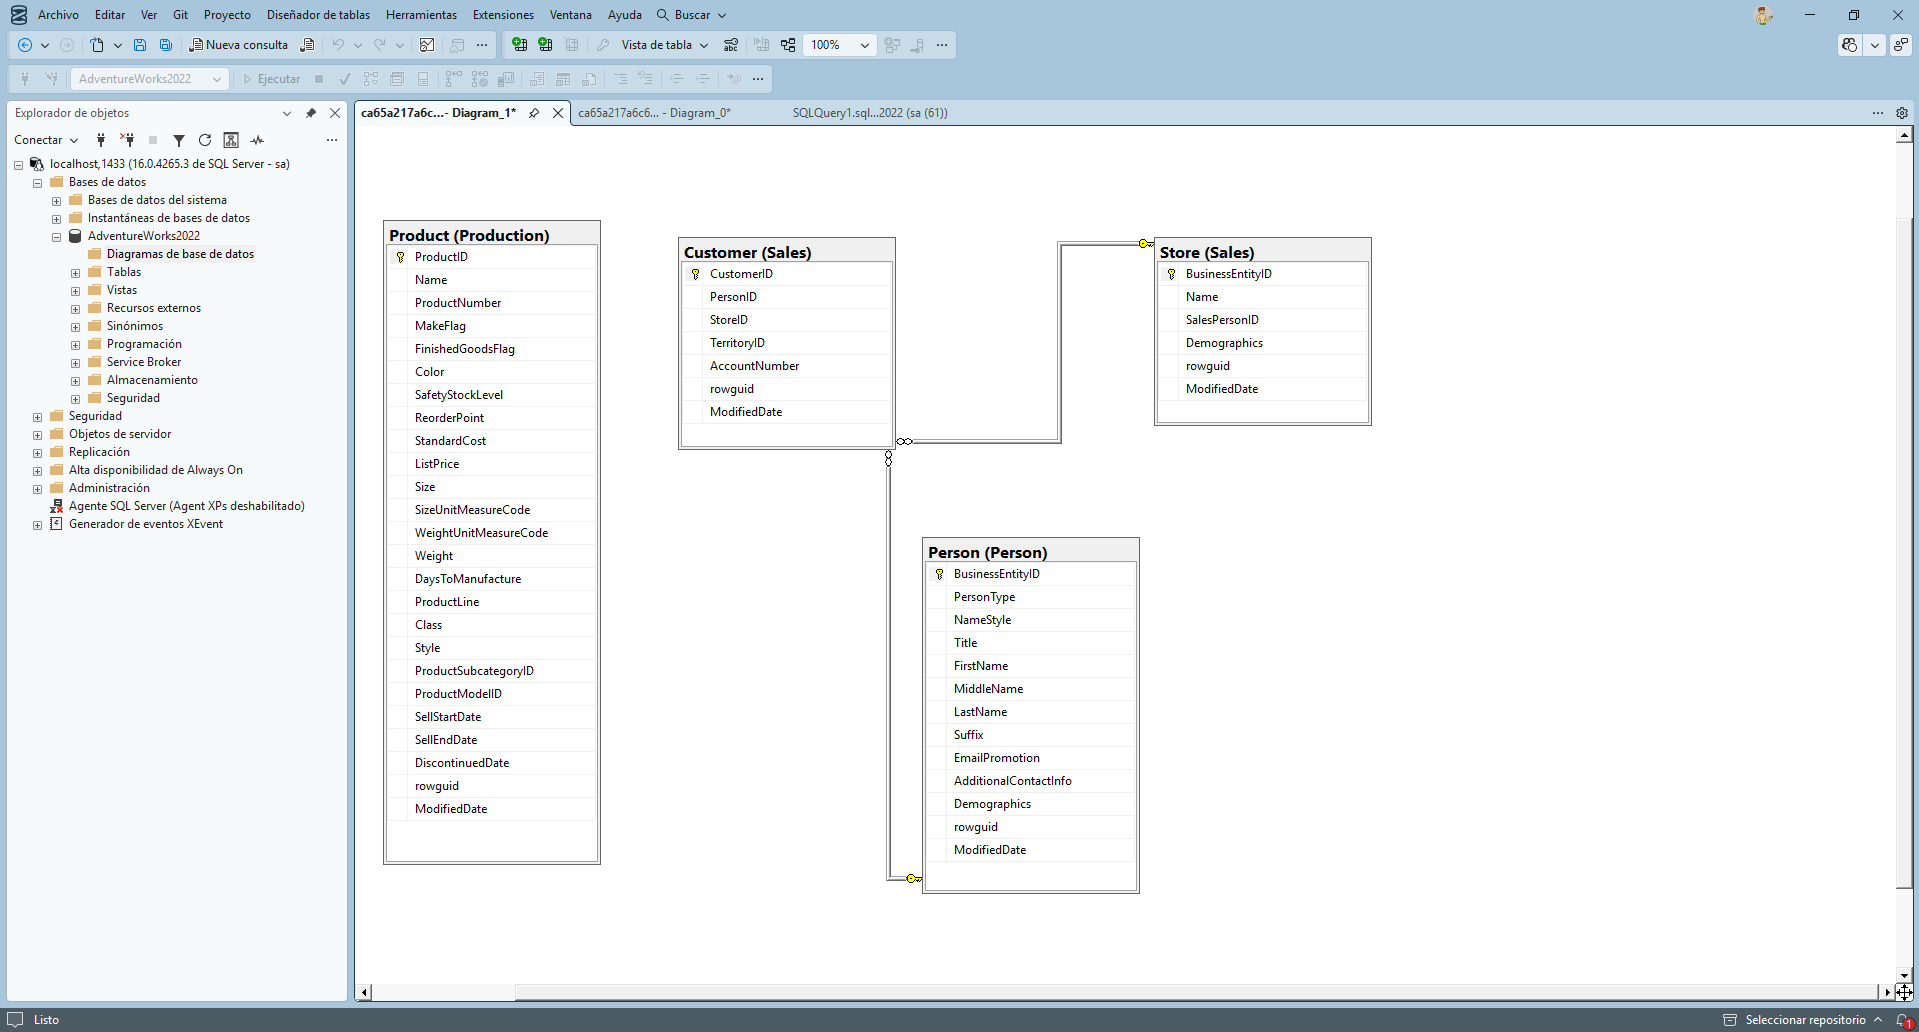
\includegraphics[width=\linewidth, height=4.2cm, keepaspectratio]{evidencia_sql2.png}\\[0.15cm]
            {\scriptsize Base de datos transaccional verificada en SQL Server.}
        \end{column}
    \end{columns}
\end{frame}

% -----------------------------------------------------------------------
% SLIDE 4: ARQUITECTURA GENERAL DE LA SOLUCIÓN
% -----------------------------------------------------------------------
\begin{frame}{Arquitectura de la Solución (4 Capas)}
    Flujo de datos desde su origen hasta su visualización, omitiendo la capa de cubos de datos (Semántica BI) según los requerimientos de la asignatura:
    
    \vspace{0.15cm}
    \begin{columns}[c]
        \begin{column}{0.48\textwidth}
            \centering
            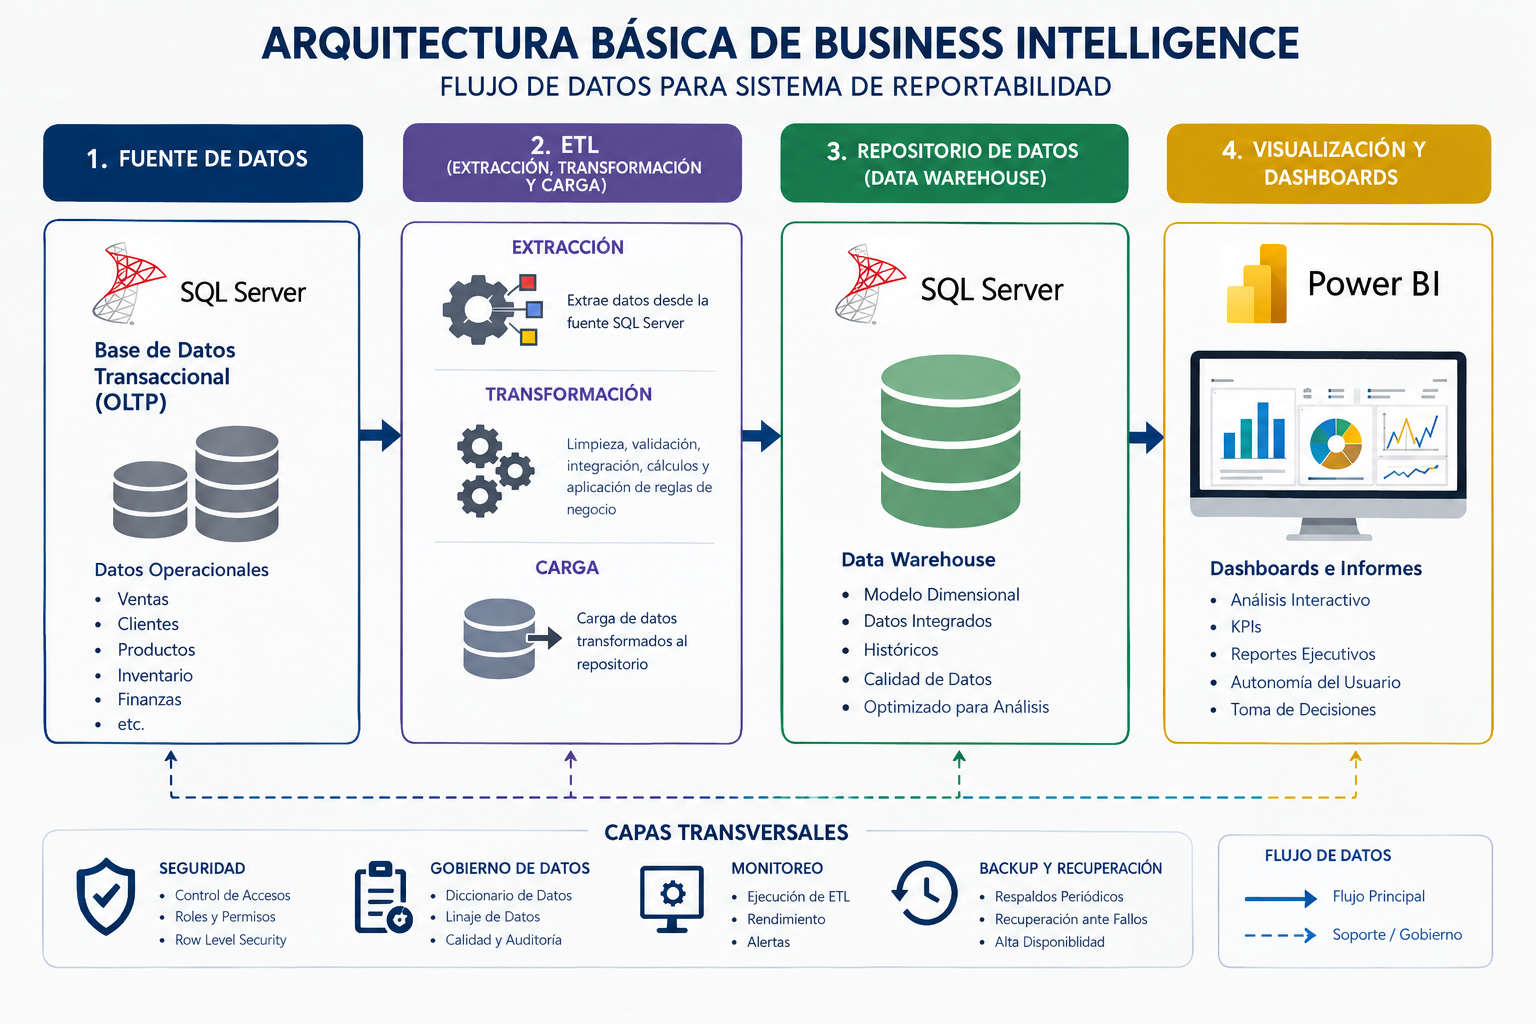
\includegraphics[width=\linewidth, height=3.5cm, keepaspectratio]{arquitectura.png}\\[0.1cm]
            {\scriptsize Flujo desacoplado en 4 capas operativas.}
        \end{column}
        
        \begin{column}{0.48\textwidth}
            \begin{block}{Las 4 Capas del Proyecto}
                \footnotesize
                \begin{enumerate}\setlength{\itemsep}{1.5pt}
                    \item \textbf{Fuente de Datos (OLTP):} Base transaccional \texttt{AdventureWorks2022}.
                    \item \textbf{ETL:} Proceso de Extracción, Transformación y Carga.
                    \item \textbf{Data Warehouse (OLAP):} Almacén estructurado en modelo dimensional.
                    \item \textbf{Visualización y Dashboards:} Tableros interactivos en Power BI.
                \end{enumerate}
            \end{block}
            
            \vspace{0.1cm}
            {\scriptsize \textcolor{gray}{\textbf{Capas Transversales:} Seguridad, Gobierno, Monitoreo y Backup.}}
        \end{column}
    \end{columns}
\end{frame}

% -----------------------------------------------------------------------
% SLIDE 5: DATA WAREHOUSE - MODELO EN ESTRELLA
% -----------------------------------------------------------------------
\begin{frame}{Data Warehouse: Modelo en Estrella}
    El almacén analítico (\texttt{AdventureWorksDW}) organiza la información en un modelo estrella desacoplado:
    
    \vspace{0.15cm}
    \begin{columns}[t]
        \begin{column}{0.48\textwidth}
            \begin{block}{7 Tablas de Dimensiones (\texttt{dw.Dim*})}
                \footnotesize
                \begin{itemize}\setlength{\itemsep}{1pt}
                    \item \textbf{\texttt{DimDate}:} Calendario diario (año, mes, trimestre).
                    \item \textbf{\texttt{DimCustomer}:} Clientes individuales y empresas.
                    \item \textbf{\texttt{DimProduct}:} Categoría, subcategoría y productos.
                    \item \textbf{\texttt{DimTerritory}:} Grupo regional, país y territorio.
                    \item \textbf{\texttt{DimLocation}:} Centros de trabajo y bodegas.
                    \item \textbf{\texttt{DimVendor}:} Proveedores de insumos.
                    \item \textbf{\texttt{DimSalesPerson}:} Vendedores asignados.
                \end{itemize}
            \end{block}
        \end{column}
        
        \begin{column}{0.48\textwidth}
            \begin{block}{5 Tablas de Hechos (\texttt{dw.Fact*})}
                \footnotesize
                \begin{itemize}\setlength{\itemsep}{2.5pt}
                    \item \textbf{\texttt{FactSales}:} Detalle de líneas de venta y montos.
                    \item \textbf{\texttt{FactWorkOrder}:} Órdenes de fabricación y rechazos.
                    \item \textbf{\texttt{FactInventory}:} Niveles de stock por bodega.
                    \item \textbf{\texttt{FactRouting}:} Horas y costos reales vs. planificados.
                    \item \textbf{\texttt{FactPurchase}:} Compras operativas a proveedores.
                \end{itemize}
            \end{block}
        \end{column}
    \end{columns}
\end{frame}

% -----------------------------------------------------------------------
% SLIDE 6: VOLUMETRÍA DEL DATA WAREHOUSE
% -----------------------------------------------------------------------
\begin{frame}{Volumetría Verificada del Almacén}
    \begin{table}[H]
    \centering
    \small
    \begin{tabularx}{0.92\textwidth}{l X r}
    \toprule
    \textbf{Tabla de Hechos} & \textbf{Qué representa cada fila} & \textbf{Filas Cargadas} \\
    \midrule
    \texttt{dw.FactSales} & Detalle de una línea de venta vendida & \textbf{121.317} \\
    \texttt{dw.FactWorkOrder} & Una orden de fabricación en planta & \textbf{72.591} \\
    \texttt{dw.FactRouting} & Una etapa u operación en la ruta de trabajo & \textbf{67.131} \\
    \texttt{dw.FactPurchase} & Una línea de compra a un proveedor & \textbf{8.845} \\
    \texttt{dw.FactInventory} & Registro de stock por producto y ubicación & \textbf{1.069} \\
    \midrule
    \textbf{Vistas \texttt{rpt}} & \textbf{Vistas analíticas creadas para Power BI} & \textbf{15 / 15} \\
    \bottomrule
    \end{tabularx}
    \end{table}
    
    \vspace{0.2cm}
    \begin{exampleblock}{Consistencia Financiera}
        \small
        El total de dinero en \texttt{FactSales} (\$109.846.381,4250) es exactamente igual al total de \texttt{SalesOrderDetail} de la base original, sin perder un solo centavo.
    \end{exampleblock}
\end{frame}

% -----------------------------------------------------------------------
% SLIDE 7: EL PROCESO ETL
% -----------------------------------------------------------------------
\begin{frame}{El Proceso ETL: Secuencia de Ejecución}
    La carga analítica completa se ejecuta con un solo comando en PowerShell (\texttt{./ejecutar-etl.ps1}), ejecutando las 5 etapas en secuencia:
    
    \vspace{0.2cm}
    \begin{columns}[t]
        \begin{column}{0.50\textwidth}
            \begin{block}{Secuencia de Carga y Transformación}
                \footnotesize
                \begin{enumerate}\setlength{\itemsep}{2.5pt}
                    \item \textbf{00. Crear Base de Datos:} Prepara el almacén \texttt{AdventureWorksDW}.
                    \item \textbf{01. Esquema OLAP:} Genera 7 dimensiones, 5 hechos, claves e índices.
                    \item \textbf{02. Carga y Limpieza:} Extrae de OLTP, normaliza datos erróneos y carga hechos.
                    \item \textbf{03. Vistas de Reportes:} Crea las 15 vistas analíticas para Power BI.
                    \item \textbf{04. Validación de Calidad:} Reconcilia filas, montos y llaves foráneas.
                \end{enumerate}
            \end{block}
        \end{column}
        
        \begin{column}{0.46\textwidth}
            \begin{exampleblock}{Características Operativas}
                \footnotesize
                \begin{itemize}\setlength{\itemsep}{2.5pt}
                    \item \textbf{Automatizado:} \texttt{ejecutar-etl.ps1} detecta SQL Server en Docker y orquesta los scripts.
                    \item \textbf{Rendimiento:} Procesa más de 270.000 filas en menos de 10 segundos.
                    \item \textbf{Tolerancia a fallos:} Usa transacciones con \texttt{ROLLBACK} ante fallas graves.
                    \item \textbf{Auditoría:} Registra fecha, duración y estado final en la tabla \texttt{dw.EtlRun}.
                \end{itemize}
            \end{exampleblock}
        \end{column}
    \end{columns}
\end{frame}

% -----------------------------------------------------------------------
% SLIDE 8: LIMPIEZA DE DATOS Y MANEJO DE ERRORES
% -----------------------------------------------------------------------
\begin{frame}{Limpieza de Datos y Tolerancia a Fallos}
    El ETL está preparado para cargar sin caerse aunque la base de pruebas contenga datos ausentes o corruptos:
    
    \vspace{0.15cm}
    \begin{columns}[t]
        \begin{column}{0.48\textwidth}
            \begin{block}{Manejo de Datos Faltantes}
                \footnotesize
                \begin{itemize}\setlength{\itemsep}{1.5pt}
                    \item \textbf{Fila comodín (-1):} Cada dimensión tiene una fila con clave \texttt{-1} para valores nulos o no informados.
                    \item \textbf{Ventas huérfanas:} Se usa \texttt{LEFT JOIN} a la orden para no descartar líneas si falta la cabecera.
                    \item \textbf{Claves inexistentes:} Si falta un producto o cliente, se asocia a \texttt{-1} en vez de abortar.
                \end{itemize}
            \end{block}
        \end{column}
        
        \begin{column}{0.48\textwidth}
            \begin{block}{Corrección de Formatos y Seguridad}
                \footnotesize
                \begin{itemize}\setlength{\itemsep}{1.5pt}
                    \item \textbf{Fechas inválidas:} Uso de \texttt{TRY\_CONVERT} para no fallar ante formatos o textos erróneos.
                    \item \textbf{Montos vacíos:} Si no viene el total, se calcula con precio, cantidad y descuento.
                    \item \textbf{Textos nulos:} Se reemplazan por etiquetas claras como \textit{"Sin país"} o \textit{"Sin nombre"}.
                    \item \textbf{Transacción segura:} Si ocurre una excepción crítica, se aplica \texttt{ROLLBACK} y registro en \texttt{EtlRun}.
                \end{itemize}
            \end{block}
        \end{column}
    \end{columns}
\end{frame}

% -----------------------------------------------------------------------
% SLIDE 9: VALIDACIÓN Y CONTROL DE CALIDAD
% -----------------------------------------------------------------------
\begin{frame}{Validación y Control de Calidad}
    \begin{columns}[c]
        \begin{column}{0.52\textwidth}
            \begin{block}{Resultados del Validador (\texttt{04\_validate.sql})}
                \small
                \begin{itemize}
                    \item Estado final de la carga: \textbf{\texttt{SUCCEEDED}}.
                    \item Resultado del validador: \textbf{\texttt{VALIDATION\_OK}}.
                    \item \textbf{Filas de hechos:} 100\% coincidentes con la fuente.
                    \item \textbf{Monto de ventas:} Reconciliado con 0 errores.
                    \item \textbf{Claves foráneas:} Cero ventas con claves perdidas.
                    \item \textbf{Vistas analíticas:} 15 vistas operativas con datos.
                \end{itemize}
            \end{block}
        \end{column}
        
        \begin{column}{0.45\textwidth}
            \begin{table}[H]
            \centering
            \scriptsize
            \begin{tabular}{l r}
            \toprule
            \textbf{Muestra de Vistas \texttt{rpt}} & \textbf{Filas Devueltas} \\
            \midrule
            \texttt{C01\_PerfilClientes} & 20 \\
            \texttt{C02\_VentasPorCliente} & 19.820 \\
            \texttt{P01\_ProduccionProducto} & 4.975 \\
            \texttt{P03\_CumplimientoOT} & 72.591 \\
            \texttt{V01\_ResumenVentas} & 38 \\
            \texttt{V02\_VentasTerritorio} & 364 \\
            \bottomrule
            \end{tabular}
            \end{table}
            \centering \scriptsize \textit{Todas las vistas entregan datos correctos para Power BI.}
        \end{column}
    \end{columns}
\end{frame}

% -----------------------------------------------------------------------
% SLIDE 10: CAPA DE REPORTABILIDAD PARA POWER BI
% -----------------------------------------------------------------------
\begin{frame}{Capa de Reportabilidad para Power BI}
    \begin{columns}[c]
        \begin{column}{0.50\textwidth}
            \begin{block}{15 Vistas en el Esquema \texttt{rpt}}
                \small
                \begin{itemize}
                    \item Cada reporte solicitado tiene su propia vista lista para usar (\texttt{rpt.C01} a \texttt{rpt.V05}).
                    \item Evita hacer relaciones o cruces complicados en Power BI.
                    \item Mejor rendimiento: Power BI solo lee la tabla analítica ya procesada y la muestra en los gráficos.
                \end{itemize}
            \end{block}
        \end{column}
        
        \begin{column}{0.48\textwidth}
            \begin{block}{Archivos de Apoyo Listos}
                \small
                \begin{itemize}
                    \item \textbf{\texttt{powerbi-tema.json}:} Plantilla de tema con la paleta de colores corporativa de los mockups.
                    \item \textbf{\texttt{powerbi-medidas.dax}:} Medidas DAX calculadas listas para usar (Ventas Totales, Ticket Promedio, Tasa de Rechazo, etc.).
                \end{itemize}
            \end{block}
        \end{column}
    \end{columns}
\end{frame}

% -----------------------------------------------------------------------
% SLIDE 11: PERSPECTIVA DE CLIENTES
% -----------------------------------------------------------------------
\begin{frame}{Catálogo de Reportes: Perspectiva de Clientes}
    \begin{columns}[c]
        \begin{column}{0.50\textwidth}
            \begin{block}{5 Reportes de Clientes}
                \small
                \begin{itemize}
                    \item \textbf{C01. Perfil de clientes:} Tipo de cliente y territorio.
                    \item \textbf{C02. Ventas por cliente:} Ranking Top 10 y ticket promedio.
                    \item \textbf{C03. Frecuencia de compra:} Clientes de una compra vs. recurrentes.
                    \item \textbf{C04. Ubicación geográfica:} Ventas por país, región y ciudad.
                    \item \textbf{C05. Clientes inactivos:} Detección de clientes sin compras recientes.
                \end{itemize}
            \end{block}
        \end{column}
        
        \begin{column}{0.48\textwidth}
            \centering
            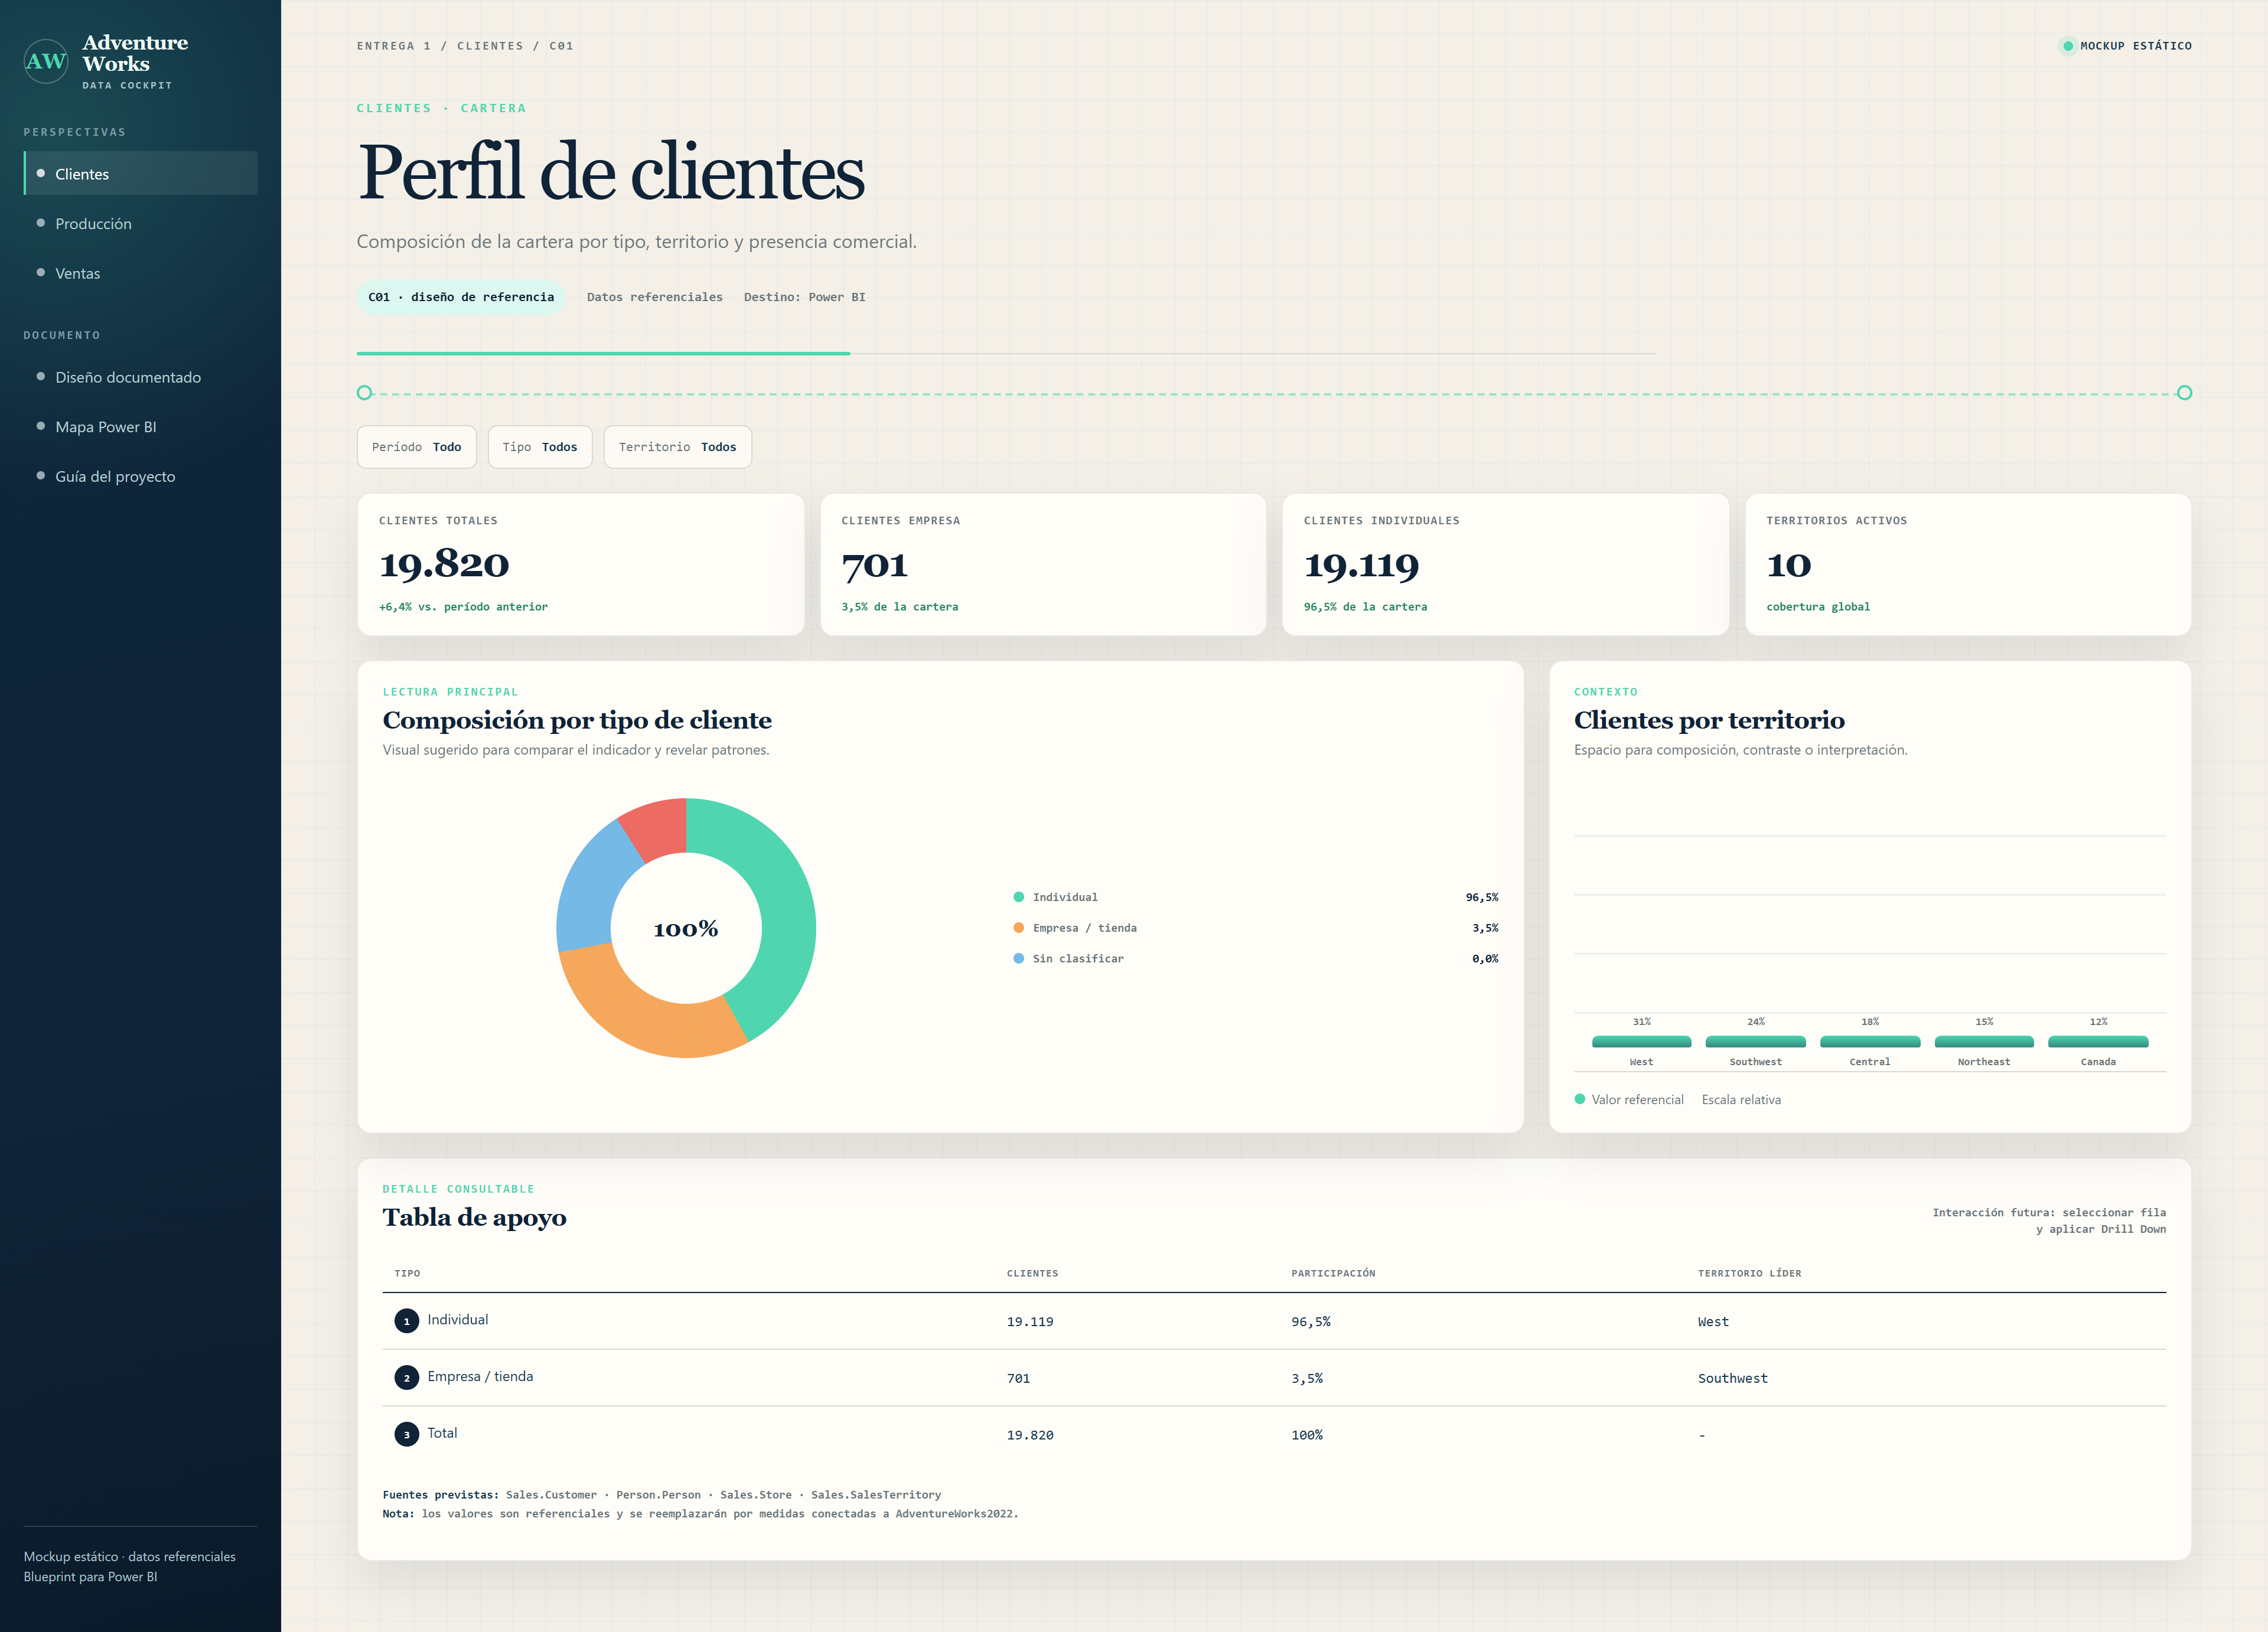
\includegraphics[width=\linewidth, height=4.2cm, keepaspectratio]{mockup_clientes_01-perfil-clientes.png}\\[0.1cm]
            {\scriptsize Mockup C01: Perfil de clientes.}
        \end{column}
    \end{columns}
\end{frame}

% -----------------------------------------------------------------------
% SLIDE 12: PERSPECTIVA DE PRODUCCIÓN
% -----------------------------------------------------------------------
\begin{frame}{Catálogo de Reportes: Perspectiva de Producción}
    \begin{columns}[c]
        \begin{column}{0.50\textwidth}
            \begin{block}{5 Reportes de Producción y Procesos}
                \small
                \begin{itemize}
                    \item \textbf{P01. Producción por producto:} Unidades y tasa de rechazo.
                    \item \textbf{P02. Inventario por ubicación:} Stock en bodega y centros de trabajo.
                    \item \textbf{P03. Cumplimiento de órdenes:} Órdenes a tiempo vs. atrasadas.
                    \item \textbf{P04. Eficiencia de rutas:} Horas y costos reales vs. planificados.
                    \item \textbf{P05. Compras a proveedores:} Unidades recibidas, rechazadas y montos.
                \end{itemize}
            \end{block}
        \end{column}
        
        \begin{column}{0.48\textwidth}
            \centering
            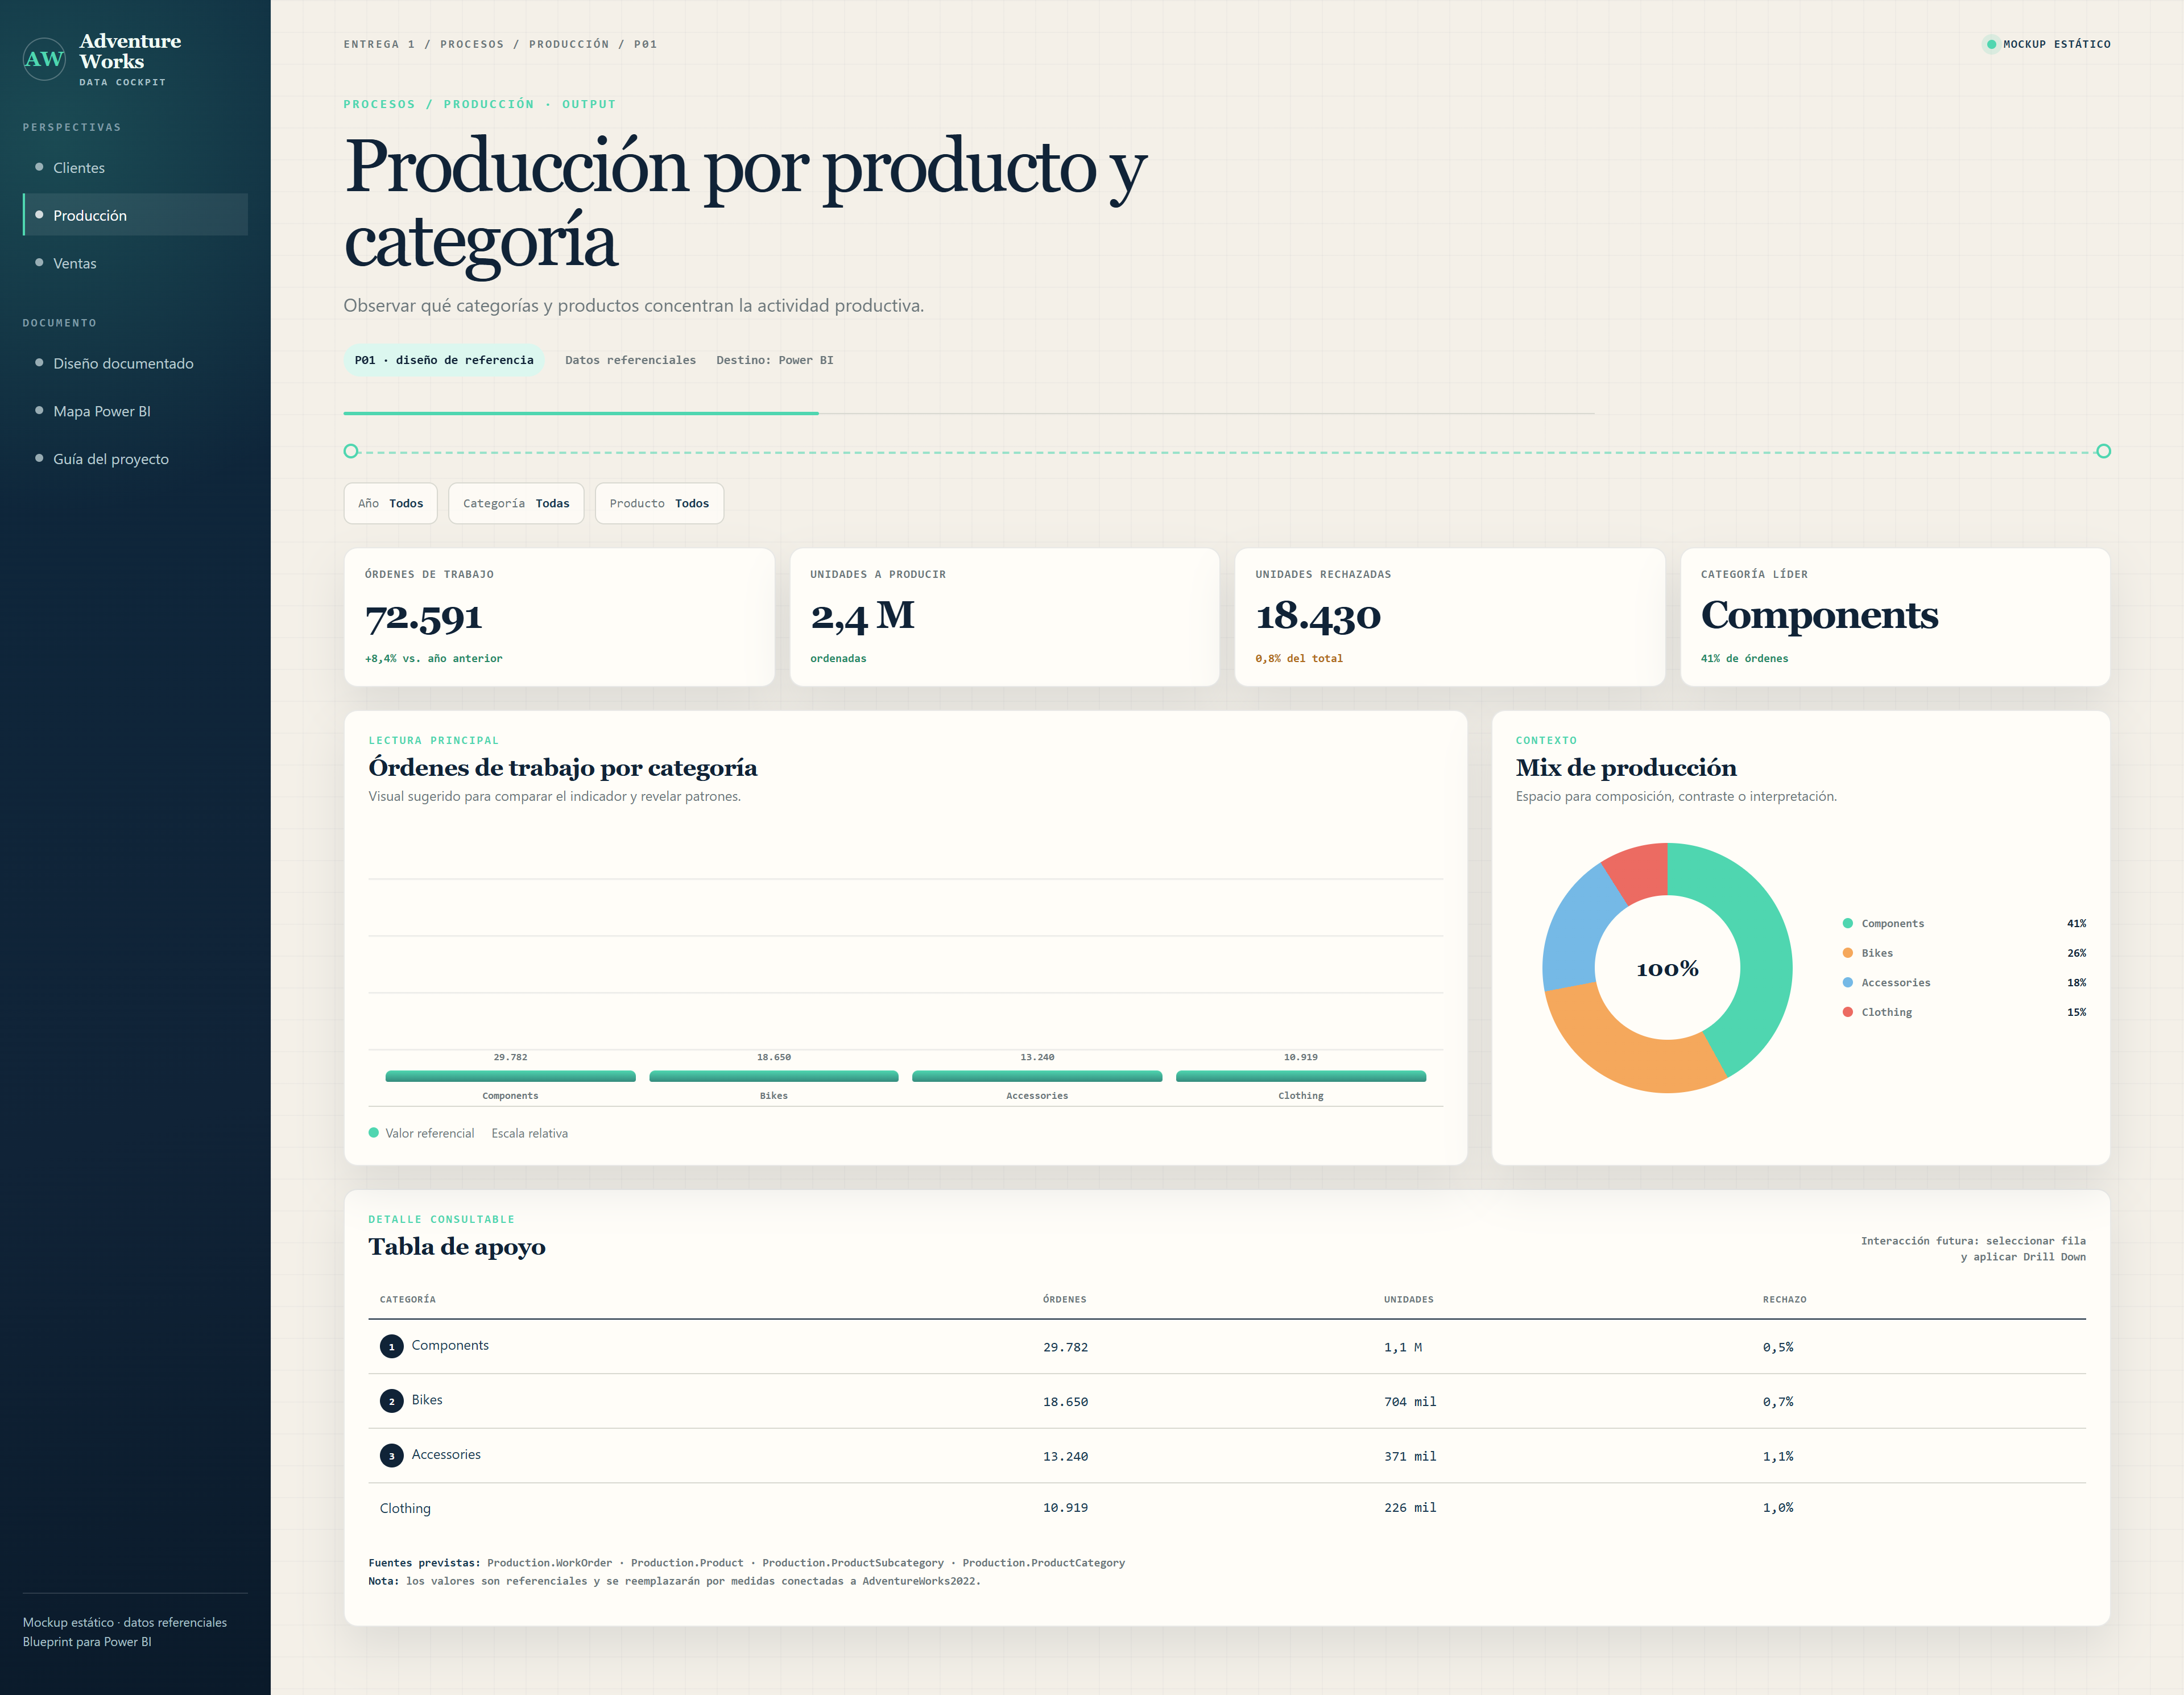
\includegraphics[width=\linewidth, height=4.2cm, keepaspectratio]{mockup_produccion_01-produccion-producto.png}\\[0.1cm]
            {\scriptsize Mockup P01: Producción por producto.}
        \end{column}
    \end{columns}
\end{frame}

% -----------------------------------------------------------------------
% SLIDE 13: PERSPECTIVA DE VENTAS
% -----------------------------------------------------------------------
\begin{frame}{Catálogo de Reportes: Perspectiva de Ventas}
    \begin{columns}[c]
        \begin{column}{0.50\textwidth}
            \begin{block}{5 Reportes Comerciales}
                \small
                \begin{itemize}
                    \item \textbf{V01. Resumen de ventas:} Ventas totales, órdenes y ticket promedio.
                    \item \textbf{V02. Ventas por territorio:} Comparación entre regiones y países.
                    \item \textbf{V03. Ventas por producto:} Categorías más vendidas y precios.
                    \item \textbf{V04. Canal de venta:} Ventas por Internet vs. distribuidores.
                    \item \textbf{V05. Desempeño de vendedores:} Ranking comercial del equipo.
                \end{itemize}
            \end{block}
        \end{column}
        
        \begin{column}{0.48\textwidth}
            \centering
            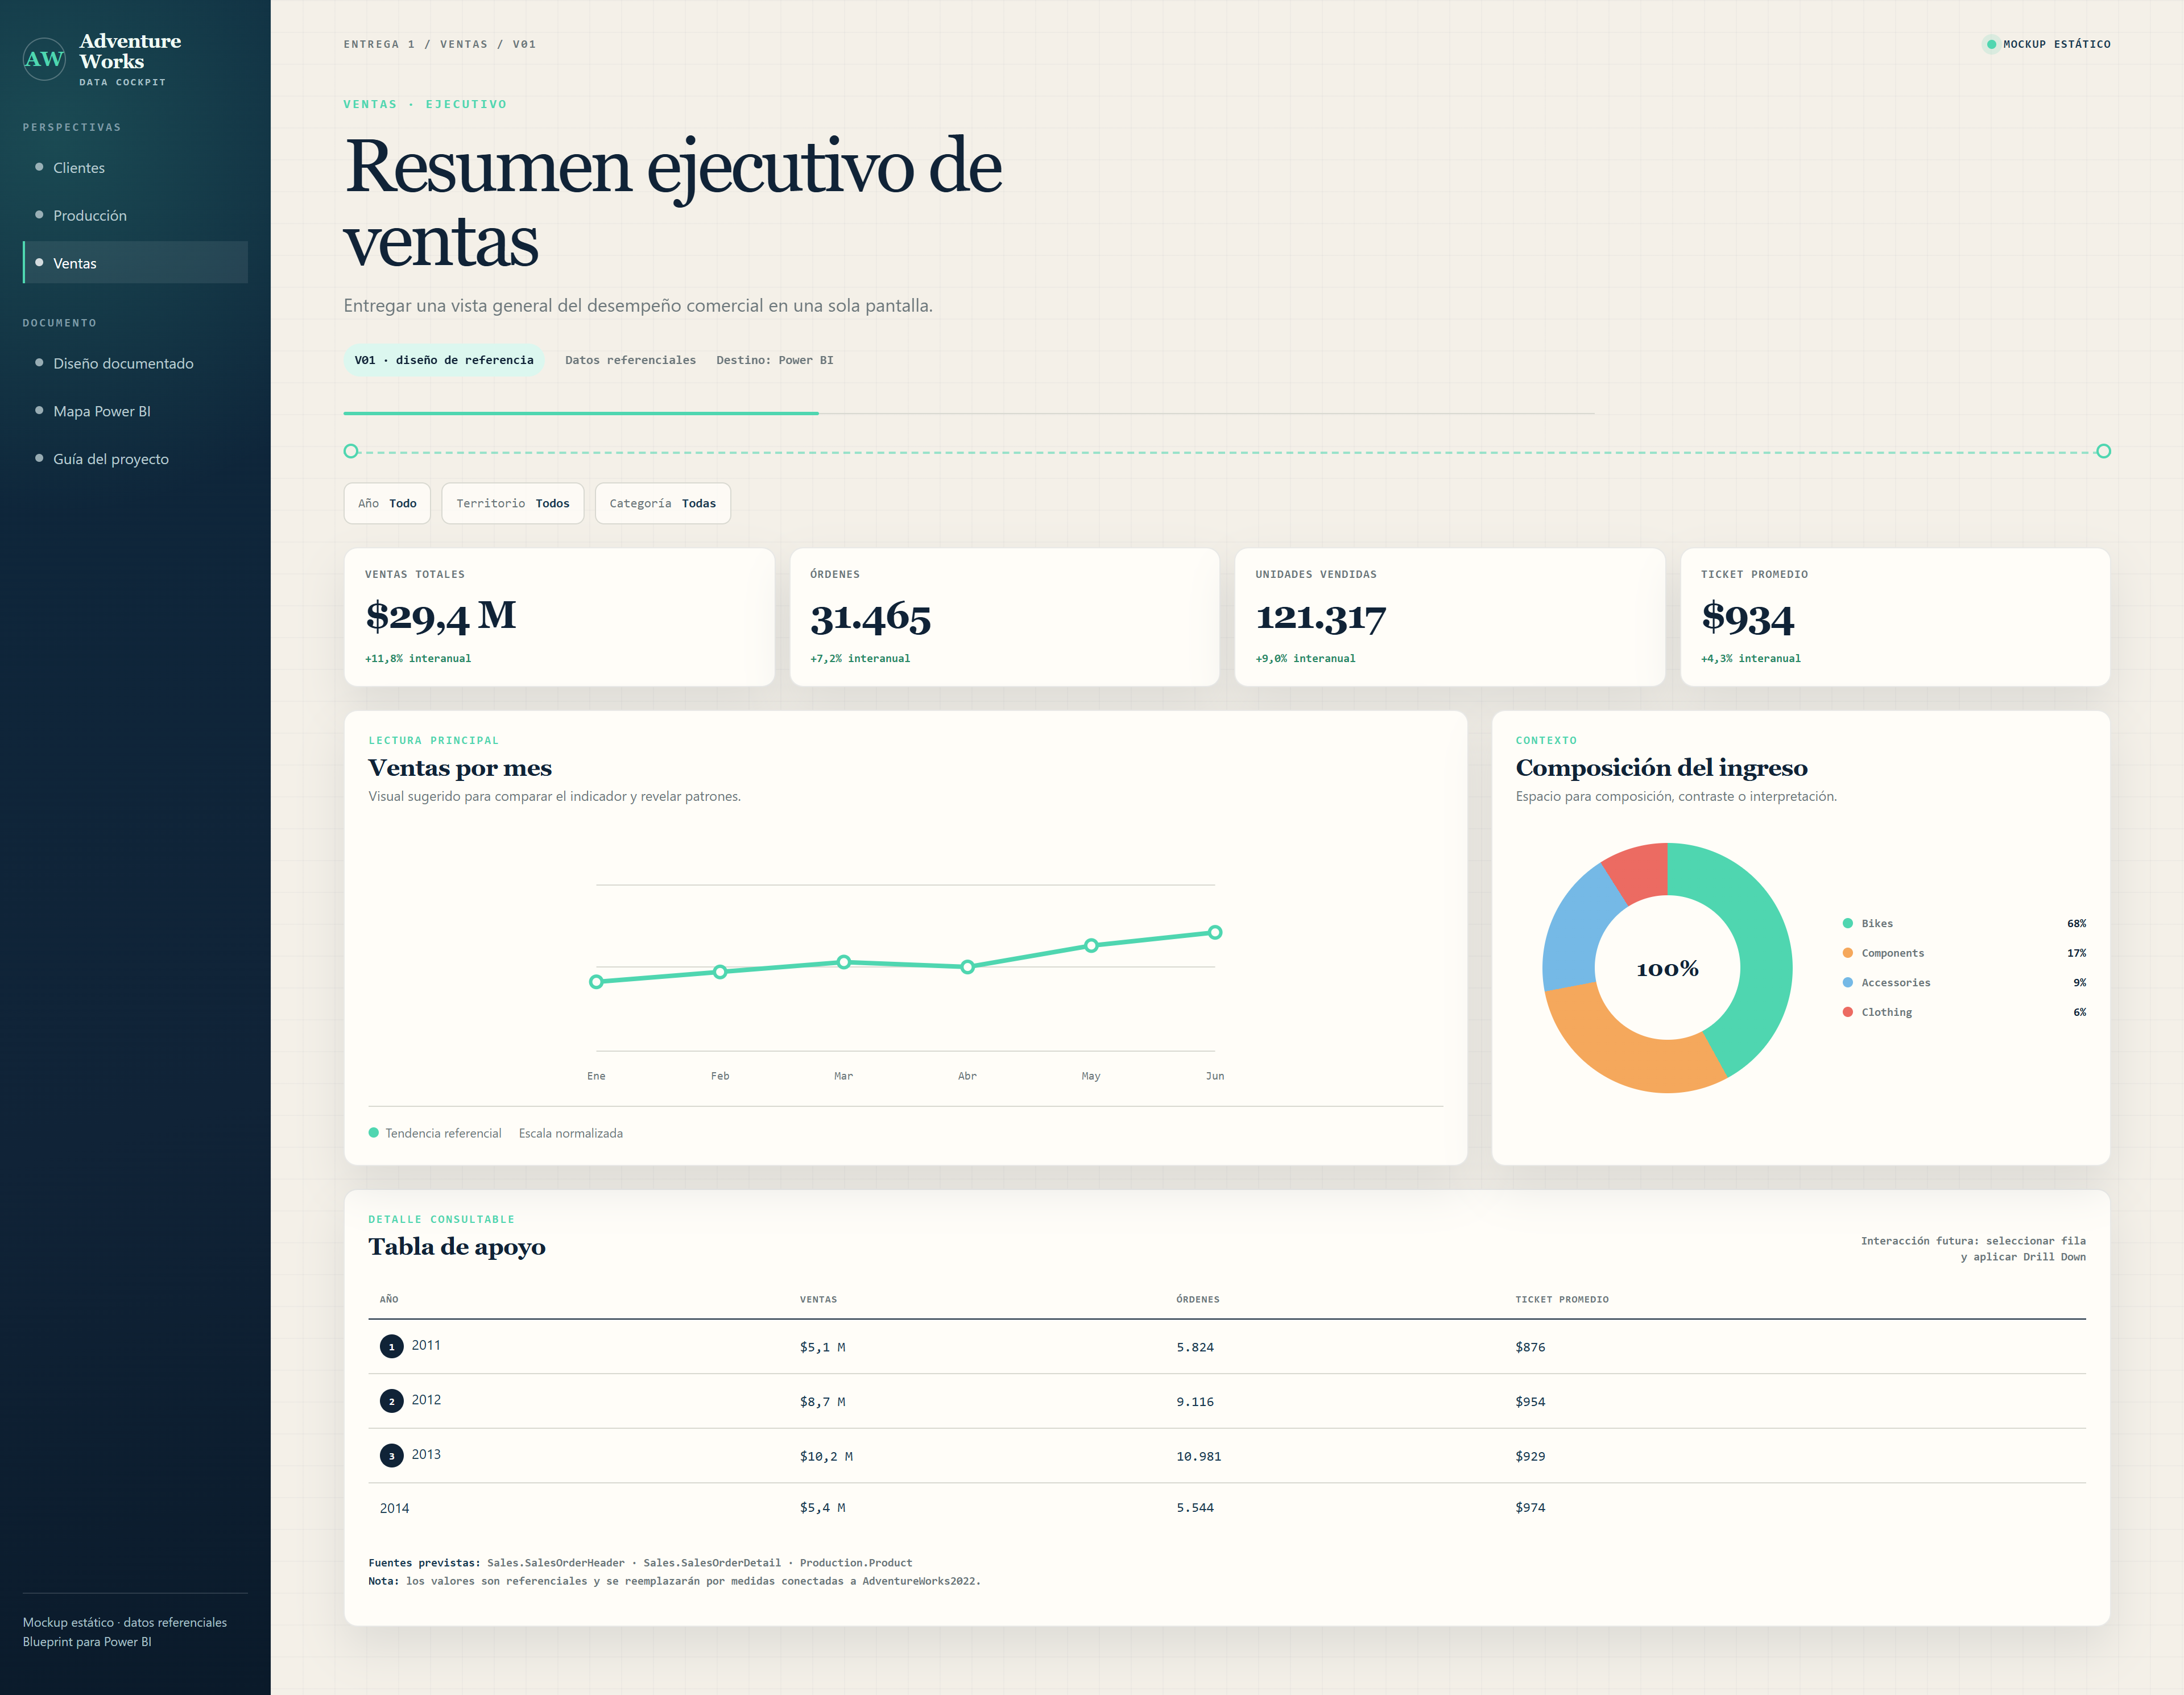
\includegraphics[width=\linewidth, height=4.2cm, keepaspectratio]{mockup_ventas_01-resumen-ventas.png}\\[0.1cm]
            {\scriptsize Mockup V01: Resumen ejecutivo comercial.}
        \end{column}
    \end{columns}
\end{frame}

% -----------------------------------------------------------------------
% SLIDE 14: NAVEGACIÓN INTERACTIVA (DRILL DOWN)
% -----------------------------------------------------------------------
\begin{frame}{Navegación Interactiva: Jerarquías de Drill Down}
    Permite profundizar desde los totales consolidados hasta el detalle específico haciendo clic directamente sobre las barras o elementos de los gráficos:
    
    \vspace{0.35cm}
    \begin{columns}[t]
        \begin{column}{0.31\textwidth}
            \begin{block}{\centering 1. Catálogo / Ventas}
                \small
                \centering
                \textbf{Categoría}\\
                $\downarrow$\\[0.08cm]
                \textbf{Subcategoría}\\
                $\downarrow$\\[0.08cm]
                \textbf{Producto}\\[0.25cm]
                \raggedright
                \footnotesize
                \textbf{Vistas:} \texttt{V03}, \texttt{P01}\\
                \textit{Bicicletas $\rightarrow$ Ruta $\rightarrow$ Modelo.}
            \end{block}
        \end{column}
        
        \begin{column}{0.31\textwidth}
            \begin{block}{\centering 2. Temporal}
                \small
                \centering
                \textbf{Año}\\
                $\downarrow$\\[0.08cm]
                \textbf{Trimestre}\\
                $\downarrow$\\[0.08cm]
                \textbf{Mes}\\[0.25cm]
                \raggedright
                \footnotesize
                \textbf{Vistas:} \texttt{V01}, \texttt{C03}\\
                \textit{2013 $\rightarrow$ Q3 $\rightarrow$ Septiembre.}
            \end{block}
        \end{column}
        
        \begin{column}{0.31\textwidth}
            \begin{block}{\centering 3. Geográfico}
                \small
                \centering
                \textbf{Región}\\
                $\downarrow$\\[0.08cm]
                \textbf{País}\\
                $\downarrow$\\[0.08cm]
                \textbf{Territorio}\\[0.25cm]
                \raggedright
                \footnotesize
                \textbf{Vistas:} \texttt{V02}, \texttt{C04}\\
                \textit{América $\rightarrow$ EE.UU. $\rightarrow$ Suroeste.}
            \end{block}
        \end{column}
    \end{columns}
\end{frame}

% -----------------------------------------------------------------------
% SLIDE 15: CONCLUSIONES Y ENTREGA 3
% -----------------------------------------------------------------------
\begin{frame}{Conclusiones y Próximo Paso}
    \begin{columns}[t]
        \begin{column}{0.48\textwidth}
            \begin{block}{Lo que se Cumplió en la Entrega 2}
                \small
                \begin{itemize}
                    \item \textbf{Base OLAP operativa:} Data Warehouse \texttt{AdventureWorksDW} con 7 dimensiones y 5 hechos.
                    \item \textbf{ETL automático:} Proceso de carga en PowerShell con limpieza ante datos erróneos.
                    \item \textbf{Vistas analíticas:} 15 vistas SQL listas y comprobadas para Power BI.
                \end{itemize}
            \end{block}
        \end{column}
        
        \begin{column}{0.48\textwidth}
            \begin{block}{Entregable 3: Reportes Implementados}
                \small
                \begin{itemize}
                    \item Conectar Power BI a las 15 vistas del Data Warehouse.
                    \item Construir los 15 tableros interactivos con los visuales y filtros aprobados en los mockups.
                    \item Validar el funcionamiento final de los gráficos y navegación \textit{Drill Down}.
                \end{itemize}
            \end{block}
        \end{column}
    \end{columns}
\end{frame}

% -----------------------------------------------------------------------
% SLIDE 16: CIERRE / PREGUNTAS
% -----------------------------------------------------------------------
\begin{frame}[plain]
    \centering
    \vspace{1.0cm}
    {\Huge \textbf{\textcolor{ucnblue}{¡Muchas Gracias!}}}\\[0.4cm]
    {\Large ¿Preguntas o Comentarios?}\\[1.2cm]
    
    \textbf{Martín Castillo Torrejón · Daniel Durán García}\\[0.15cm]
    \footnotesize Ingeniería de Datos y Big Data · Universidad Católica del Norte\\[0.4cm]
    \scriptsize \textcolor{gray}{\url{https://github.com/Charmandiox9/Ing.-Datos-y-Big-Data}}
\end{frame}

\end{document}